\documentclass[a4paper, 11pt]{article}

\usepackage[utf8]{inputenc}
\usepackage[english]{babel}

\usepackage{hyperref}

\usepackage{standalone}

\usepackage{lscape}

\usepackage{multirow}
\usepackage{graphicx}
\usepackage{subfig}
\usepackage{tikz}
\usetikzlibrary{decorations.pathreplacing}
\usepackage{floatrow}
\captionsetup{labelsep=period}

\usepackage{amsmath}

\usepackage{fullpage}

\begin{document}
	\begin{centering}
		\Large{\textbf{Progress Report}}\\
		\large{\today}
~\\
		Oussama ENNAFII\\
		Directors: Cl\'ement Mallet \& Florent Lafarge \\
		Advisor: Arnaud Le Bris \\

	\end{centering}


	\section{The Dataset:}
	\subsection{Considerations:}
~\\

	We have decided earlier in June to work on Nantes and Dijon in addition to
	Elancourt. As I explained later, the $3DS$ data for these regions are not
	well formated so that I can retrieve the building entities. In order to
	establish first a whole pipeline. I will deal with those regions later using
	the $CityGML$ data. In consequence, I will continue to work on Elancourt
	only, for now.\\

	I have also relabelled the zone I had labelled before. That is due to the fact
	that the taxonomy has evolved during the annotation. I have used $QGIS$ to
	annotate buildings' projected facets based on errors they showed.\\

	\subsection{Annotated errors:}
~\\


	The errors have been subdivided, based on the labelling, into three classes:

	\begin{itemize}
		\item[-] Unqualified Building Errors (\textit{c.f.} figure.~\ref{fig::samples} -- (i).): Concerns the buildings that will not
		be taken into consideration,
		\item[-] Building Errors (\textit{c.f.} figure.~\ref{fig::samples} -- (ii).):
		encompasses the errors that affect the whole building (corrensponds roughly to $LoD0$ and $LoD1$ errors),
		\item[-] Facet Errors (\textit{c.f.} figure.~\ref{fig::samples} -- (iii).):
		concerns errors affecting only a facet.
	\end{itemize}

	\thisfloatsetup{heightadjust=object}
	\begin{figure}
		\begin{center}
			\ffigbox{
				\ffigbox[\FBwidth]{
					\begin{subfloatrow}[4]
						\captionsetup{labelformat=brace, justification=raggedright}
						\ffigbox[\FBwidth]{\caption{Half Building: only a portion of the building is reconstructed.}\label{fig::half_building}}{\fbox{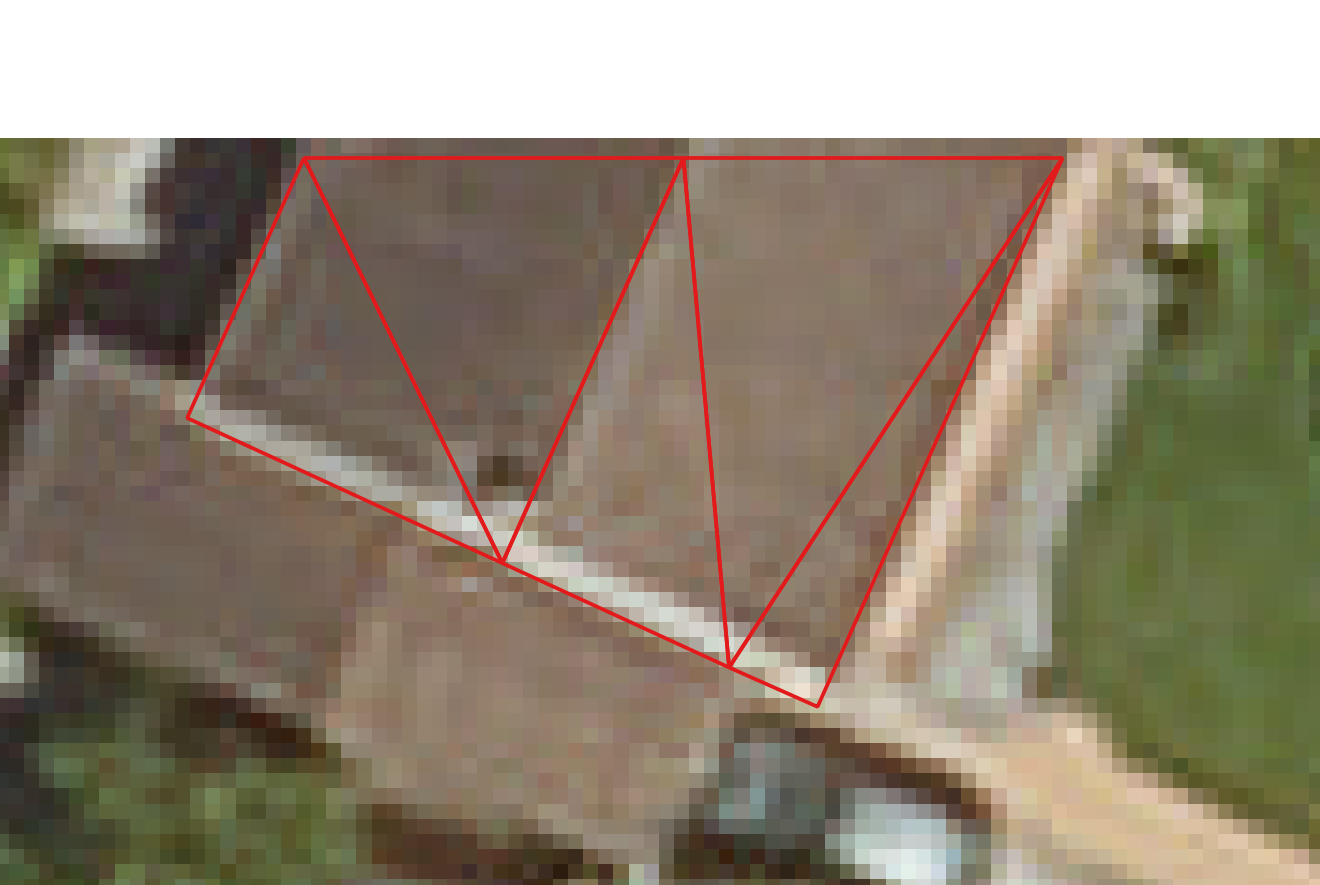
\includegraphics[width=.24\textwidth]{../images/raster/Unqualified_Errors/half_building}}}
						\ffigbox[\FBwidth]{\caption{Changed Building: the building has changed so we cannot qualify it.}\label{fig::changed}}{\fbox{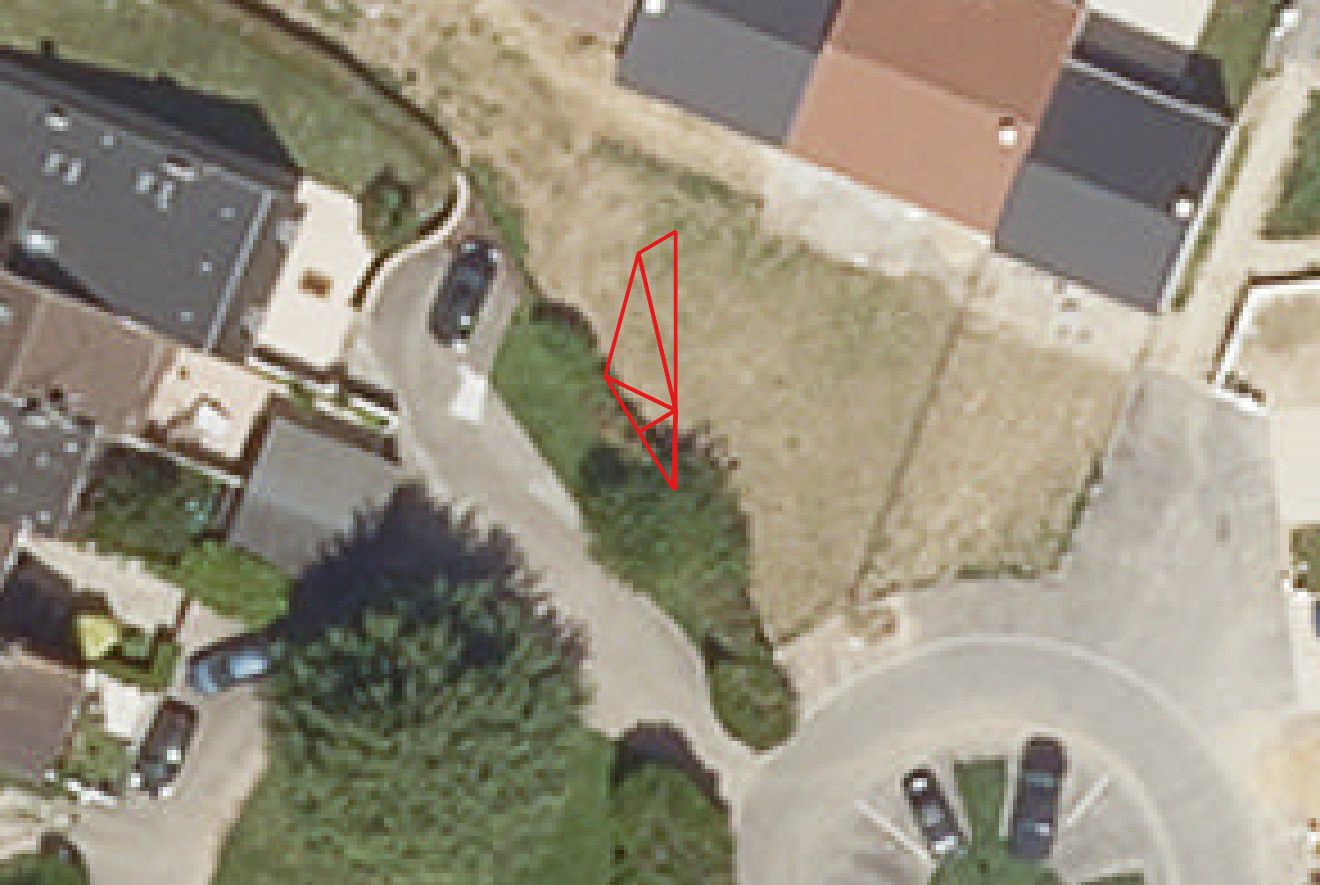
\includegraphics[width=.24\textwidth]{../images/raster/Unqualified_Errors/changed}}}
						\ffigbox[\FBwidth]{\caption{Occlusion: the building is occluded by vegetation here.}\label{fig::occlusion}}{\fbox{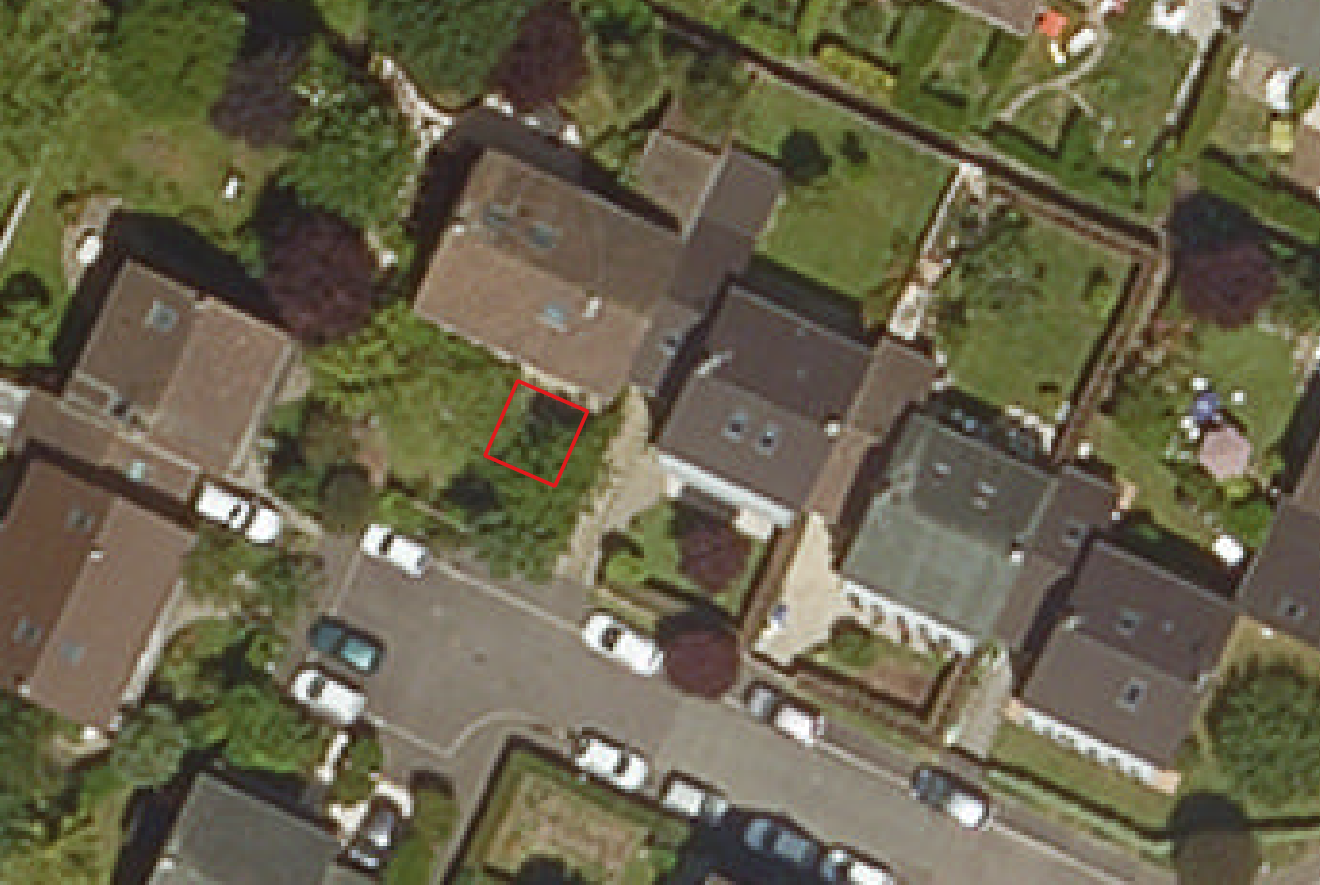
\includegraphics[width=.24\textwidth]{../images/raster/Unqualified_Errors/occlusion}}}
						\ffigbox[\FBwidth]{\caption{Unknown: Unknown shape that cannot be verified on the ground.}\label{fig::unknown}}{\fbox{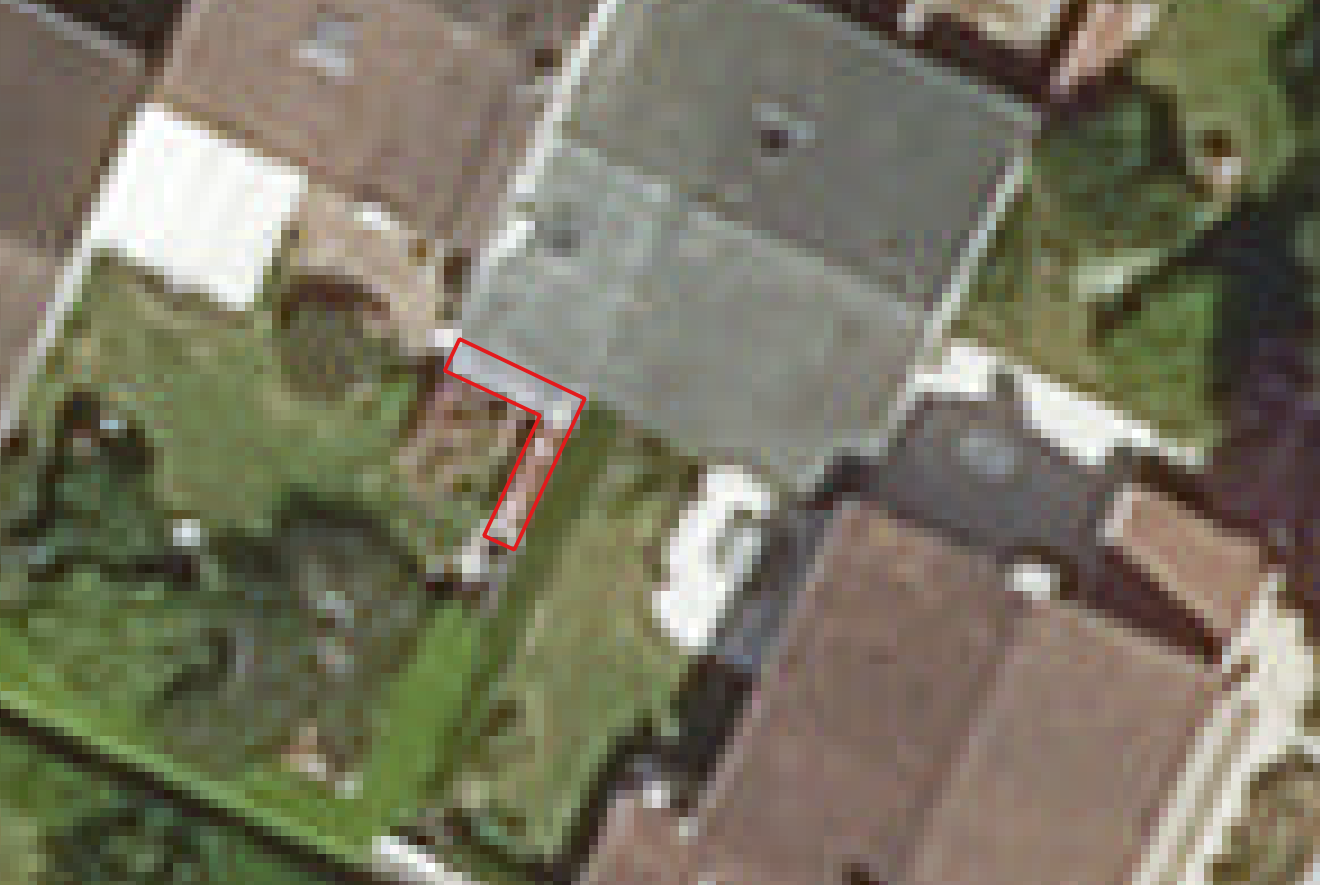
\includegraphics[width=.24\textwidth]{../images/raster/Unqualified_Errors/unknown}}}
					\end{subfloatrow}
				}
				{
					\caption*{(i). Samples of Unqualified building errors.}
				}
				\ffigbox[\FBwidth]
				{
					\begin{subfloatrow}[4]
						\captionsetup{labelformat=brace, justification=raggedright}
						\ffigbox[\FBwidth]{\caption{Under Segmentation: Two or more buildings grouped into one.}\label{fig::under_bul}}{\fbox{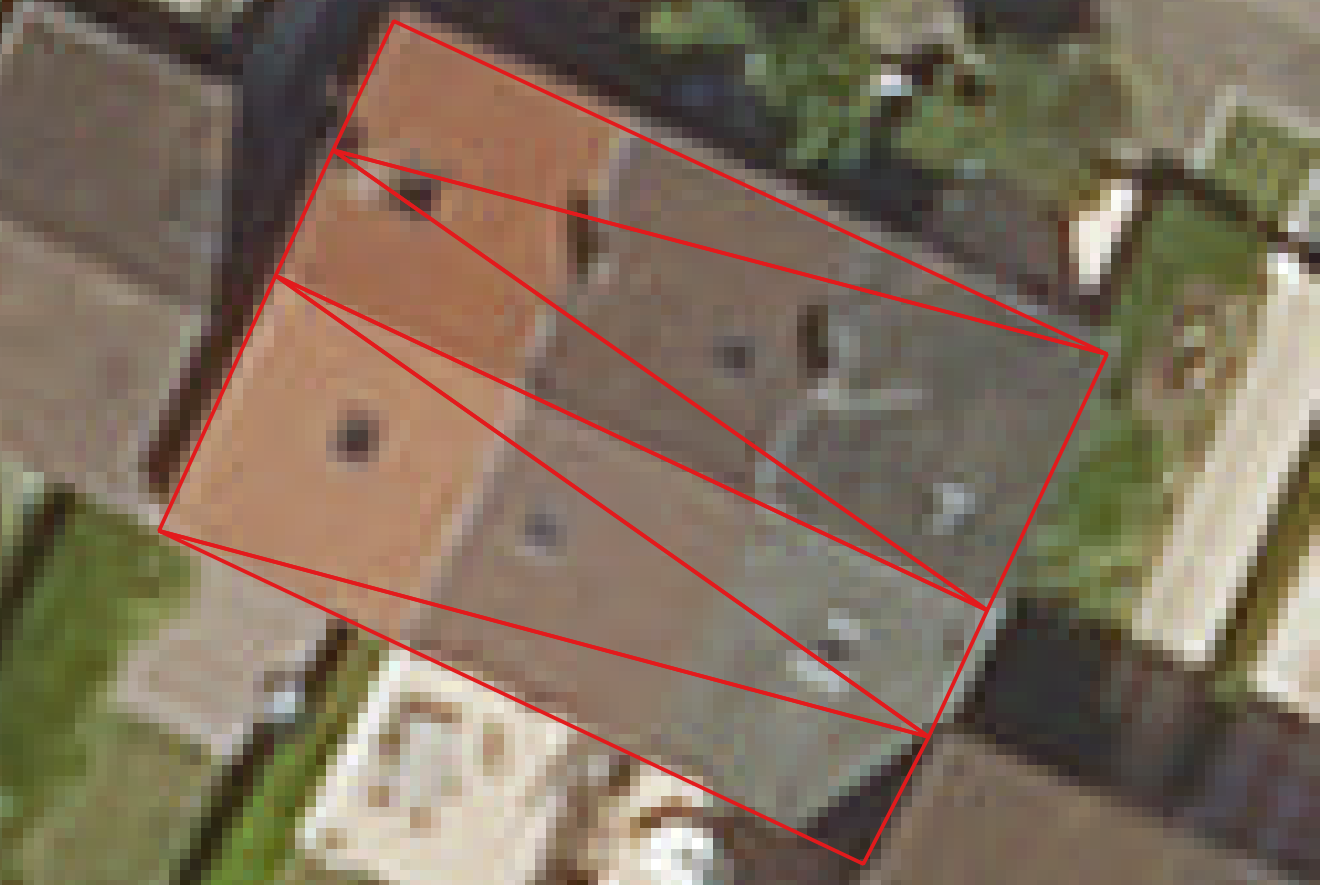
\includegraphics[width=.24\textwidth]{../images/raster/Building_Errors/under_segmentation}}}
						\ffigbox[\FBwidth]{\caption{Over segmentation: One building segmented into two or more buildings.}\label{fig::over_bul}}{\fbox{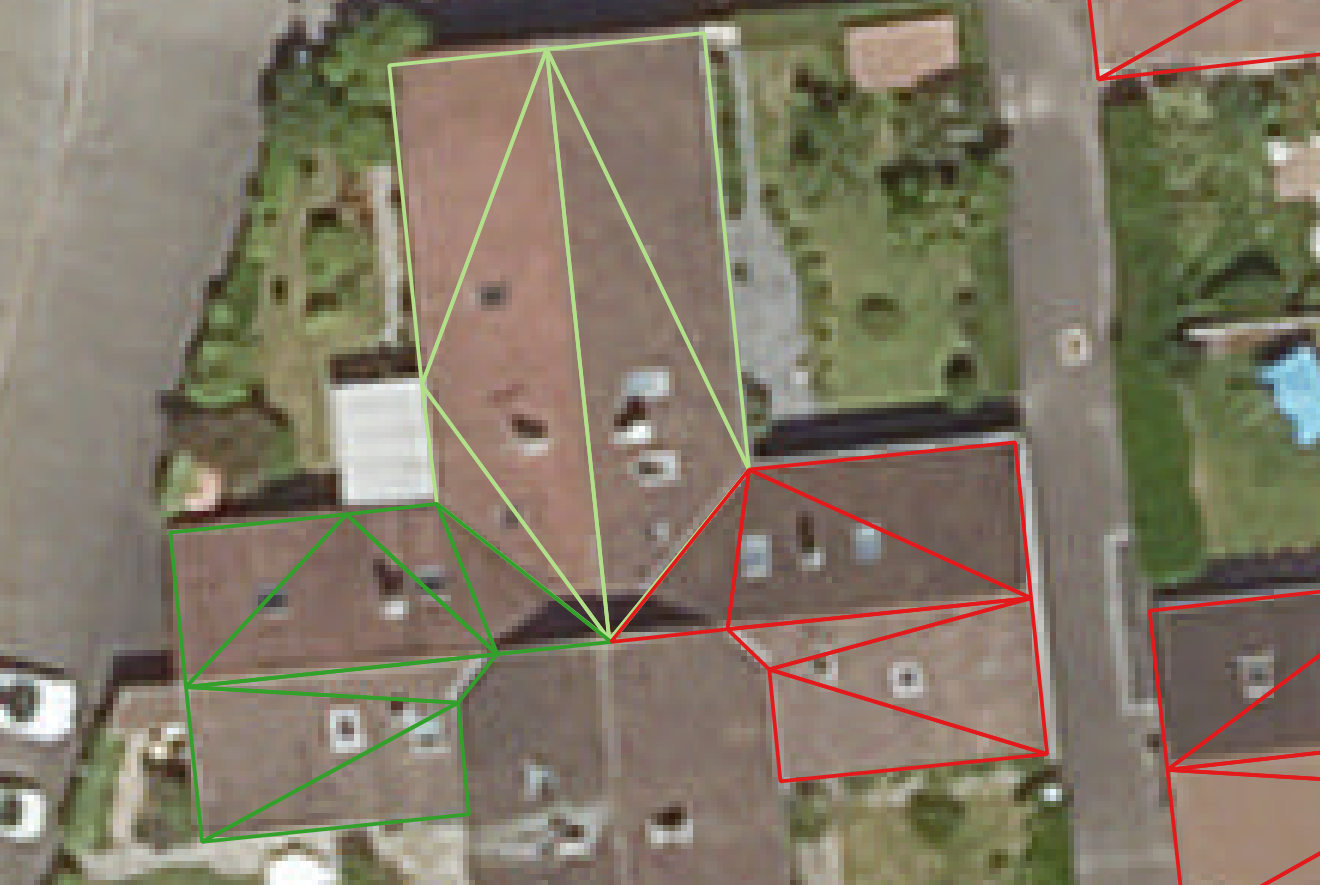
\includegraphics[width=.24\textwidth]{../images/raster/Building_Errors/over_segmentation}}}
						\ffigbox[\FBwidth]{\caption{Footprint: Wrong building footprint.}\label{fig::footprint}}{\fbox{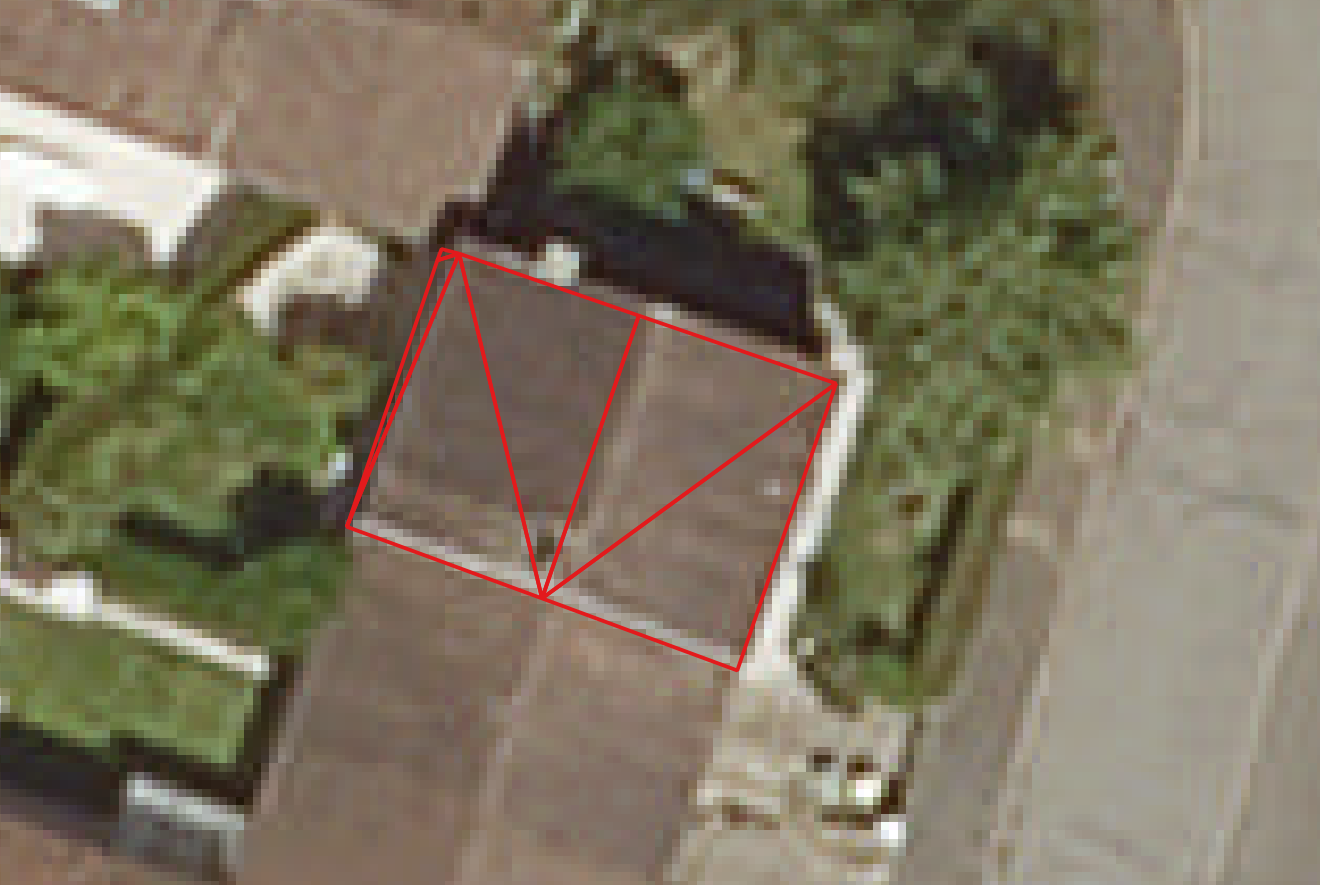
\includegraphics[width=.24\textwidth]{../images/raster/Building_Errors/footprint}}}
						\ffigbox[\FBwidth]{\caption{Altitude: Wrong building height.}\label{fig::too_low}}{\fbox{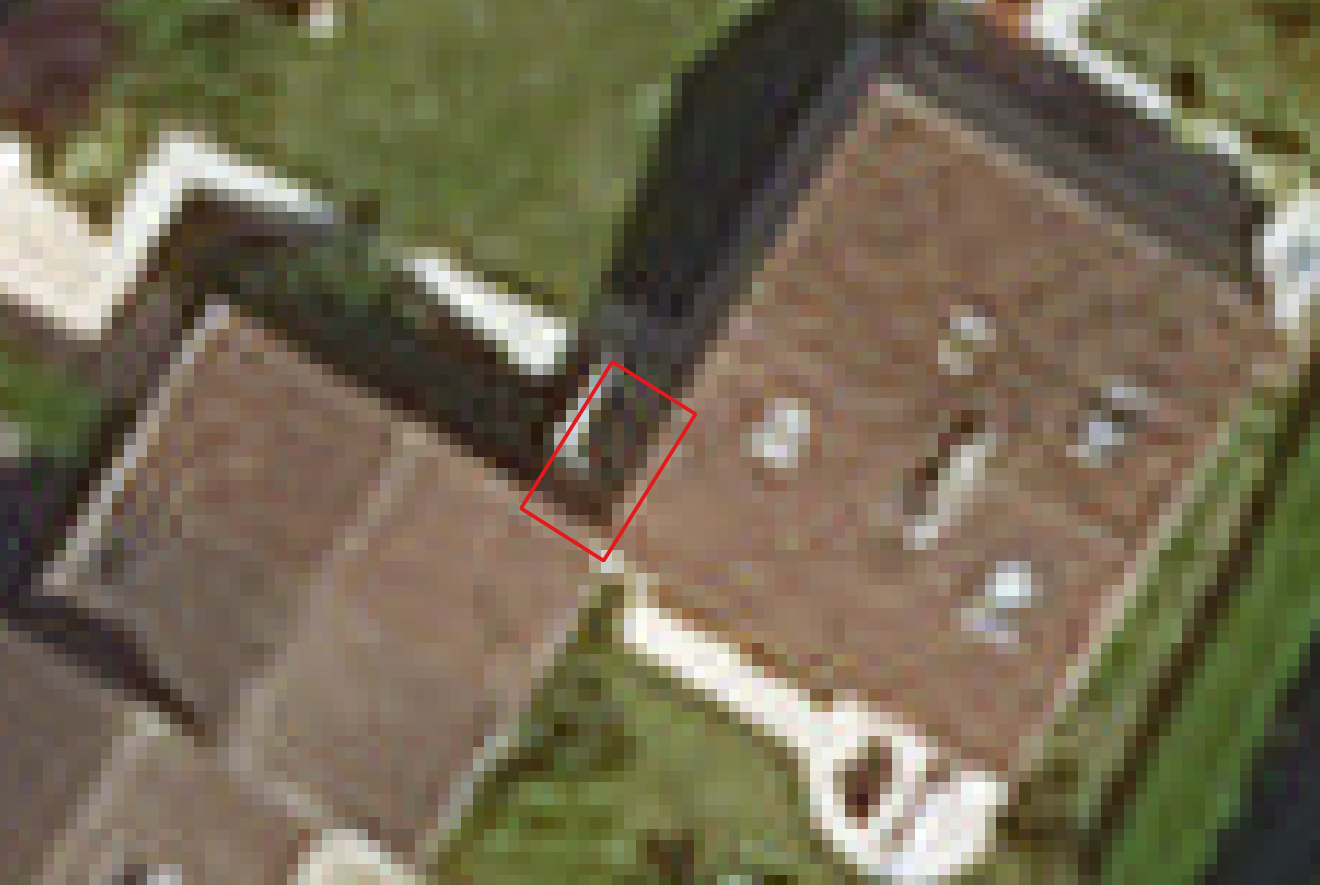
\includegraphics[width=.24\textwidth]{../images/raster/Building_Errors/altimetric}}}
					\end{subfloatrow}
				}
				{
					\caption*{(ii). Samples of Building errors.}
				}
				\ffigbox[\FBwidth]
				{
					\begin{subfloatrow}[4]
						\captionsetup{labelformat=brace, justification=raggedright}
						\ffigbox[\FBwidth]{\caption{Under Segmentation: Two facets or more grouped into one.}\label{fig::under_fac}}{\fbox{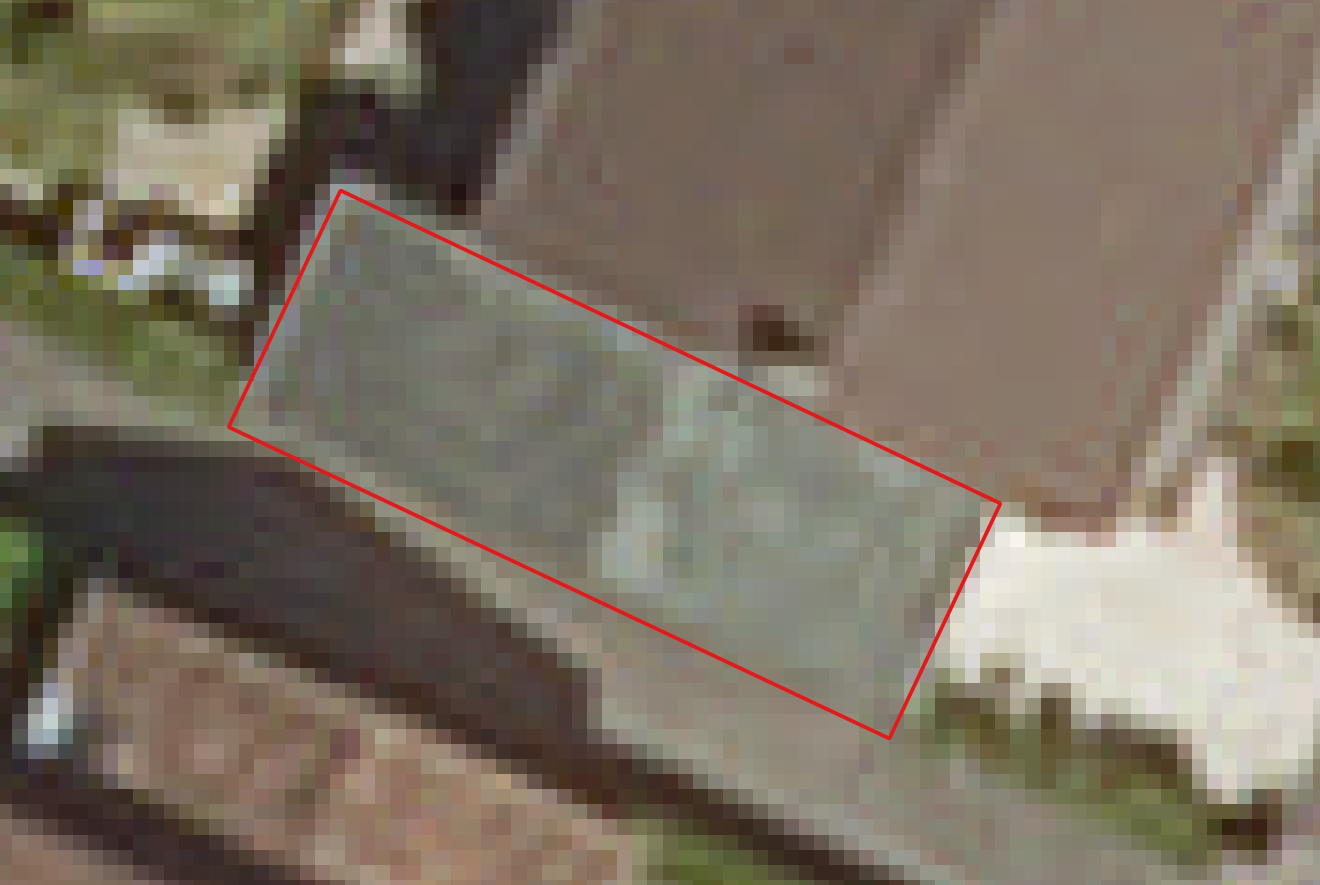
\includegraphics[width=.24\textwidth]{../images/raster/Facet_Errors/under_segmentation}}}
						\ffigbox[\FBwidth]{\caption{Over segmentation: One facet segemented into two or more facets.}\label{fig::over_fac}}{\fbox{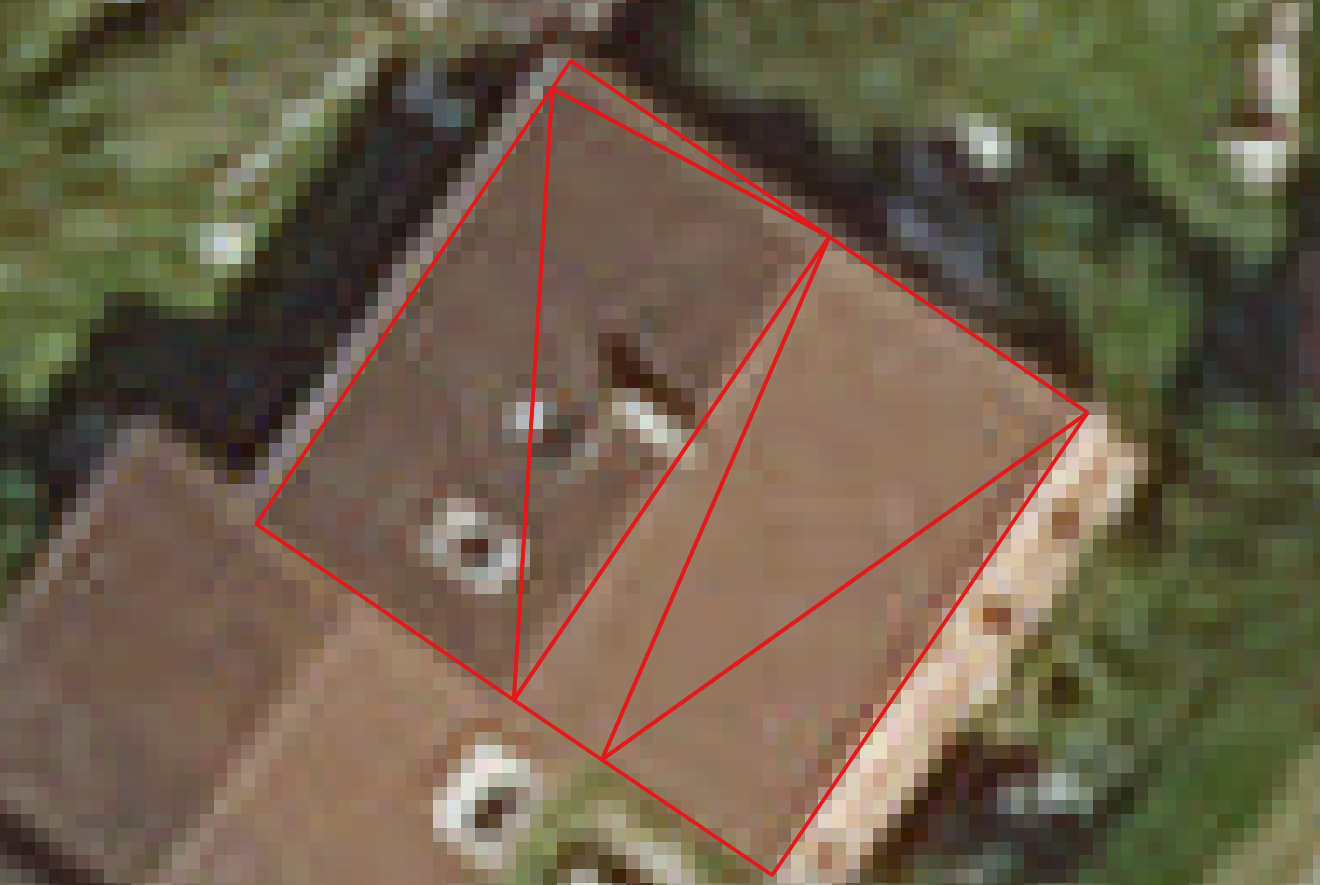
\includegraphics[width=.24\textwidth]{../images/raster/Facet_Errors/over_segmentation}}}
						\ffigbox[\FBwidth]{\caption{Mis Segmentation: Facet edges do not correspond to real ones.}\label{fig::mis}}{\fbox{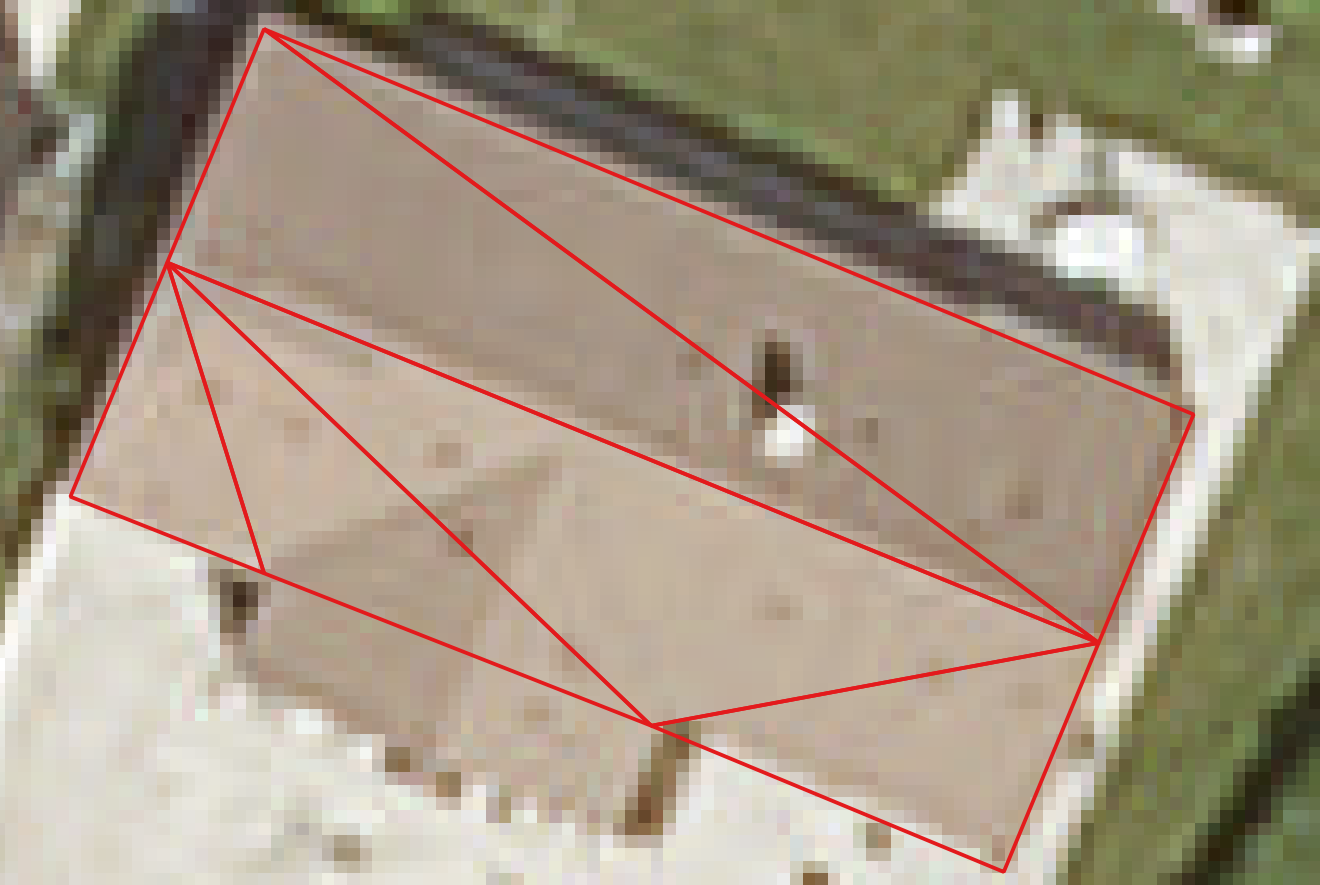
\includegraphics[width=.24\textwidth]{../images/raster/Facet_Errors/mis_segmentation}}}
						\ffigbox[\FBwidth]{\caption{Slope: Wrong facet slope.}\label{fig::slope}}{\fbox{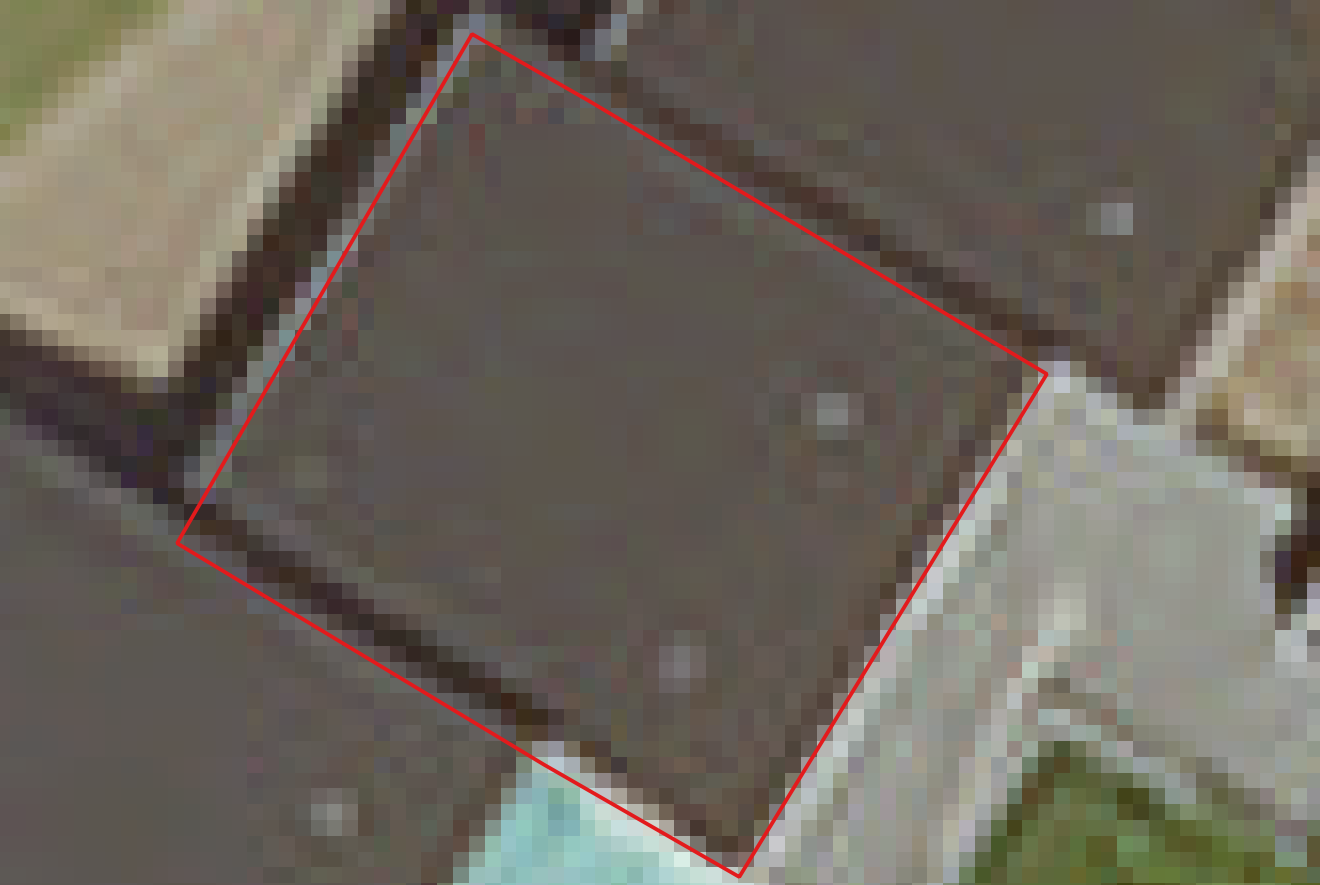
\includegraphics[width=.24\textwidth]{../images/raster/Facet_Errors/slope}}}
					\end{subfloatrow}
				}
				{
					\caption*{(iii). Samples of Facet errors.}
				}
			}
			{
				\caption{\label{fig::samples}Illustration of errors per class.}
			}
		\end{center}
	\end{figure}
	\clearpage

	Here are some statistics over the labelled dataset (\textit{c.f.} figure.~\ref{fig::dataset}) comprizing $502$ buildings:

	\thisfloatsetup{heightadjust=object}
	\begin{figure}
		\ffigbox[\FBwidth]
		{
			\begin{subfloatrow}[3]
				\captionsetup{labelformat=brace, justification=raggedright}
				\ffigbox[\FBwidth]
				{
					\fbox{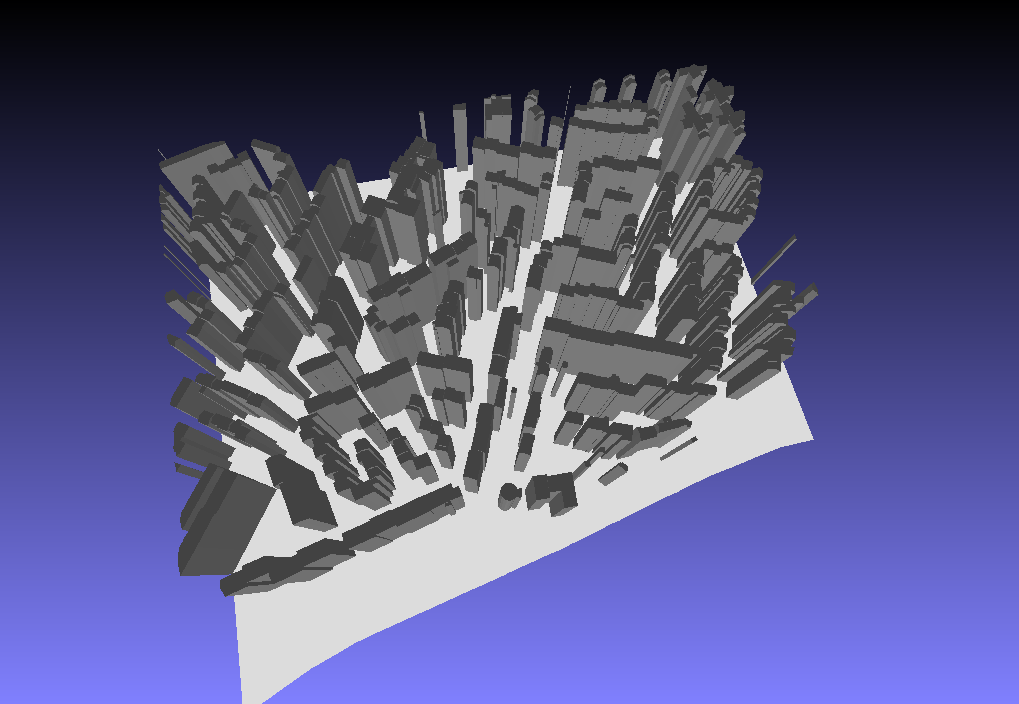
\includegraphics[width=.29\textwidth]{../images/raster/snapshot00}}
				}
				{
					\caption{Snapshot of the 3D scene.}\label{fig::snapshot}
				}
				\ffigbox[\FBwidth]
				{
					\fbox{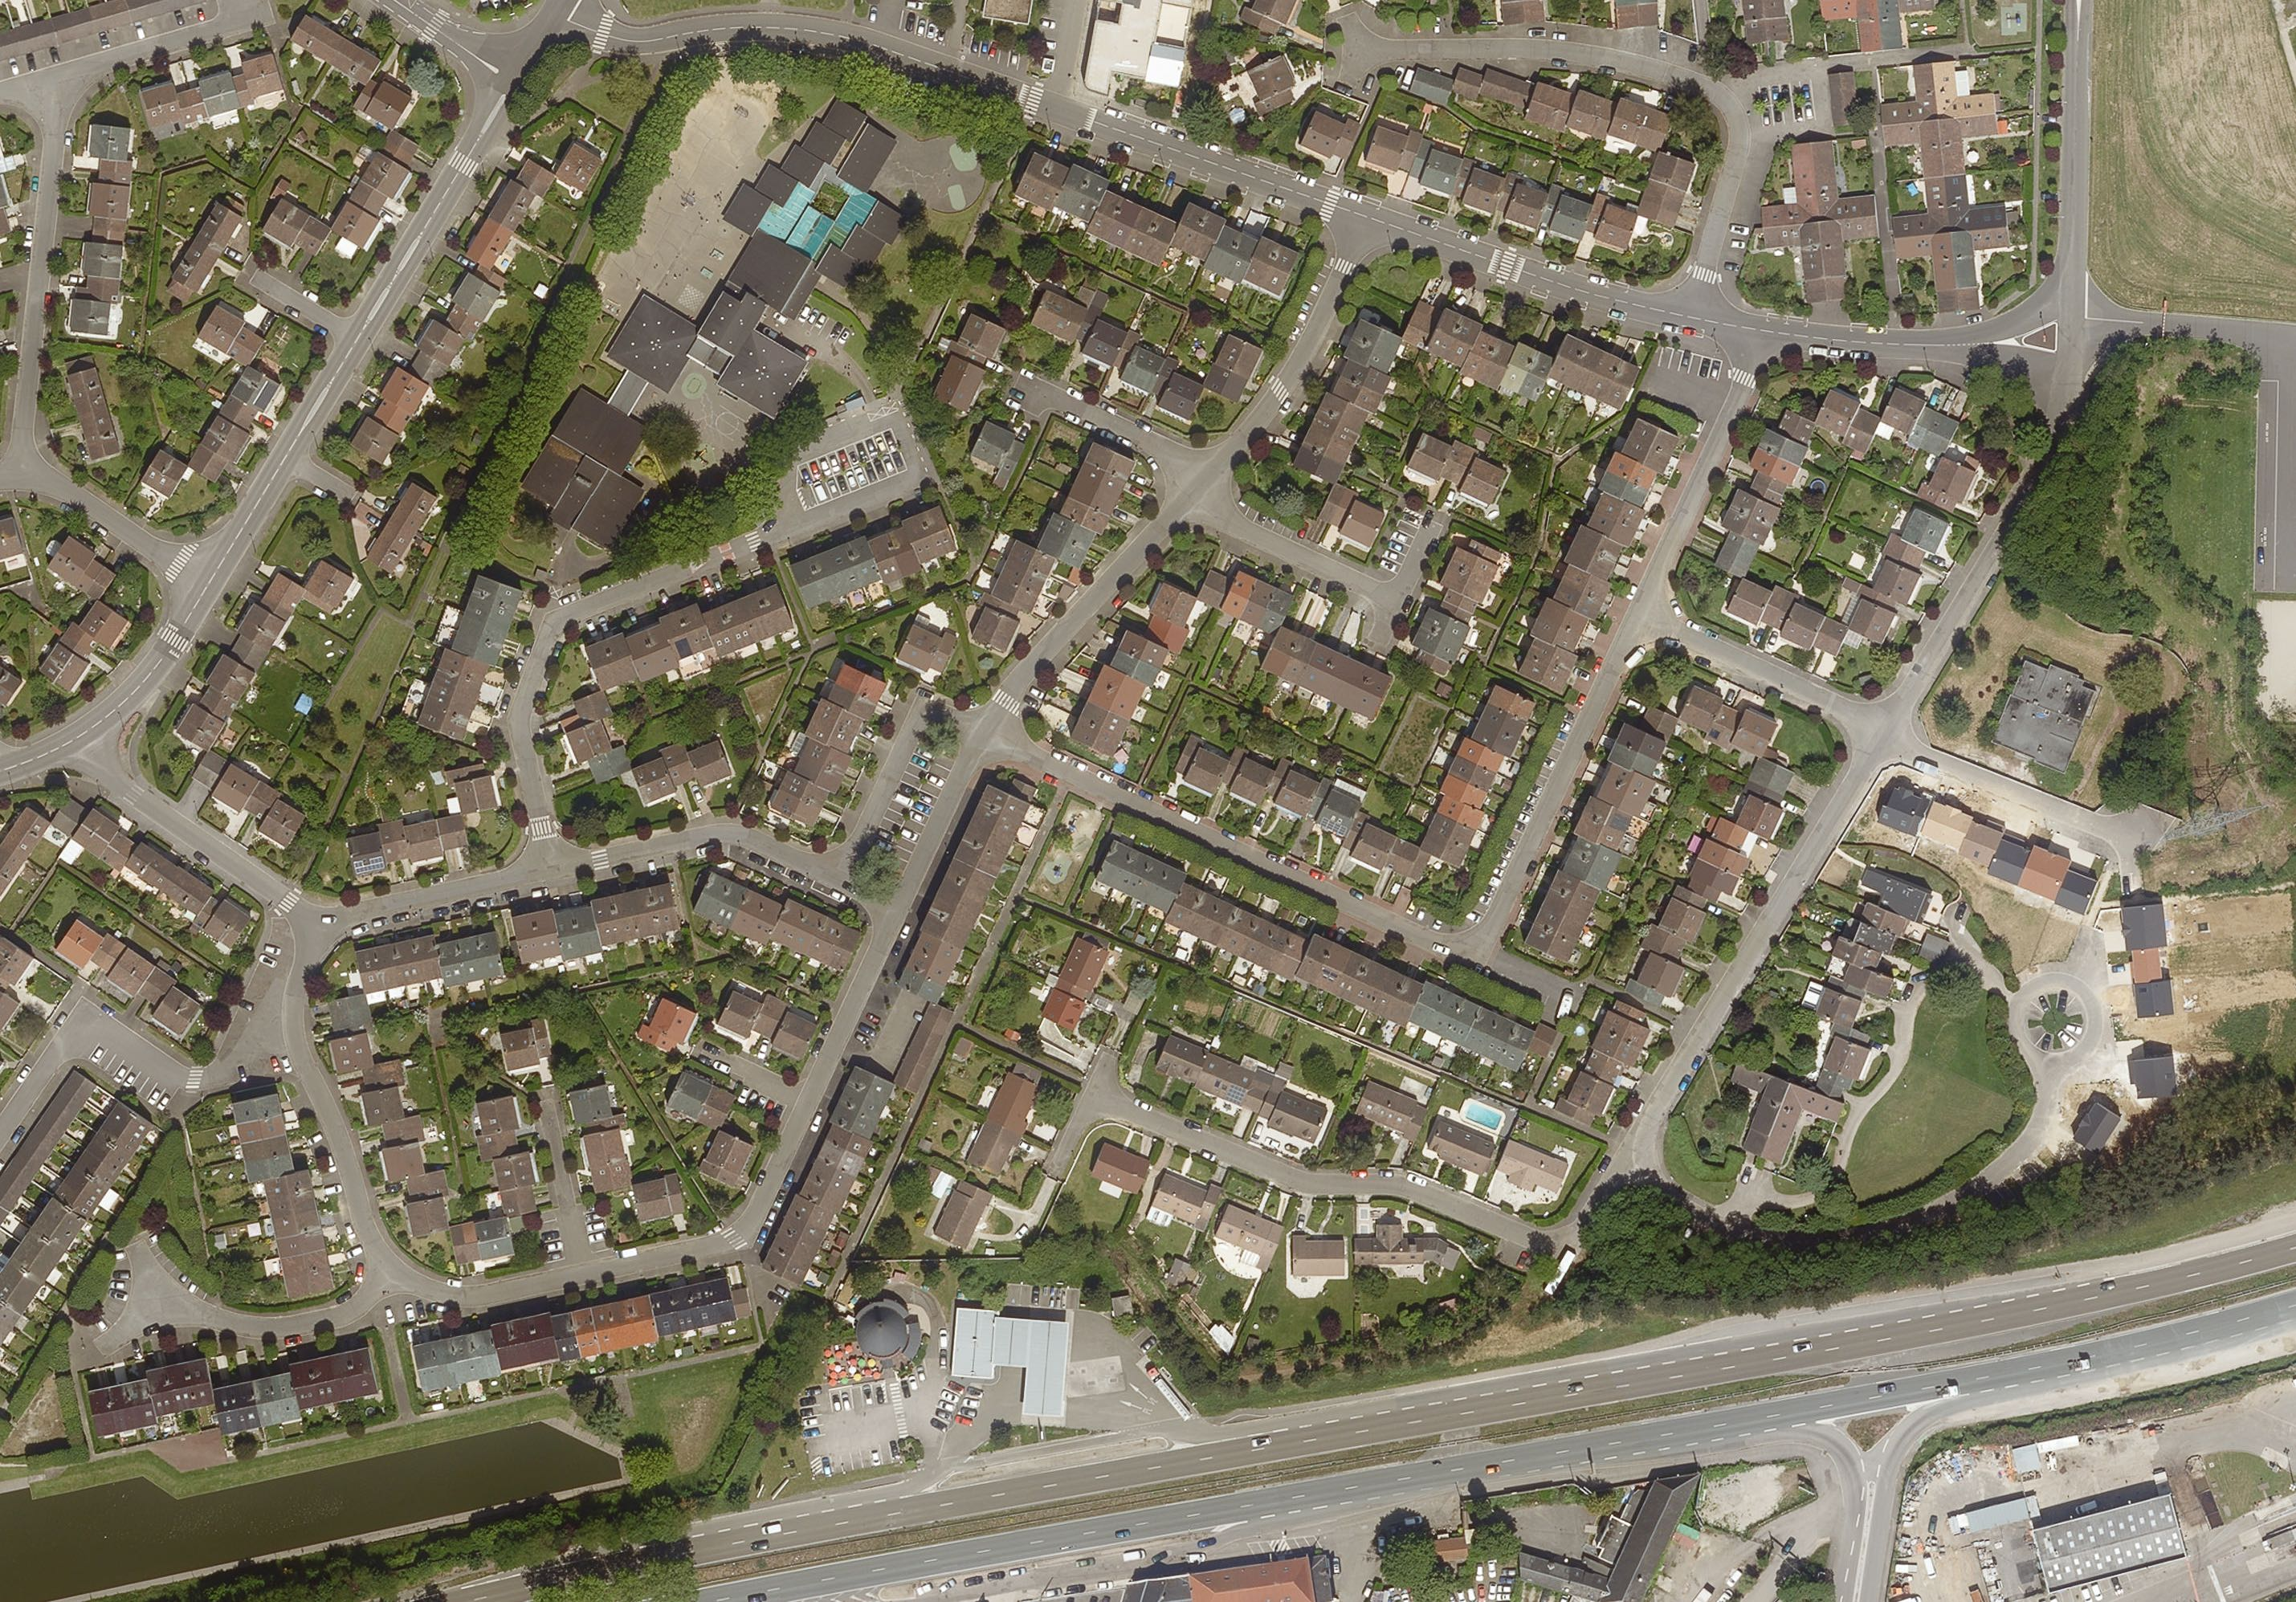
\includegraphics[width=.285\textwidth]{../images/raster/orthoimage}}
				}
				{
					\caption{Orthoimage corresponding to the scene.}\label{fig::ortho}
				}
				\ffigbox[\FBwidth]
				{
					\fbox{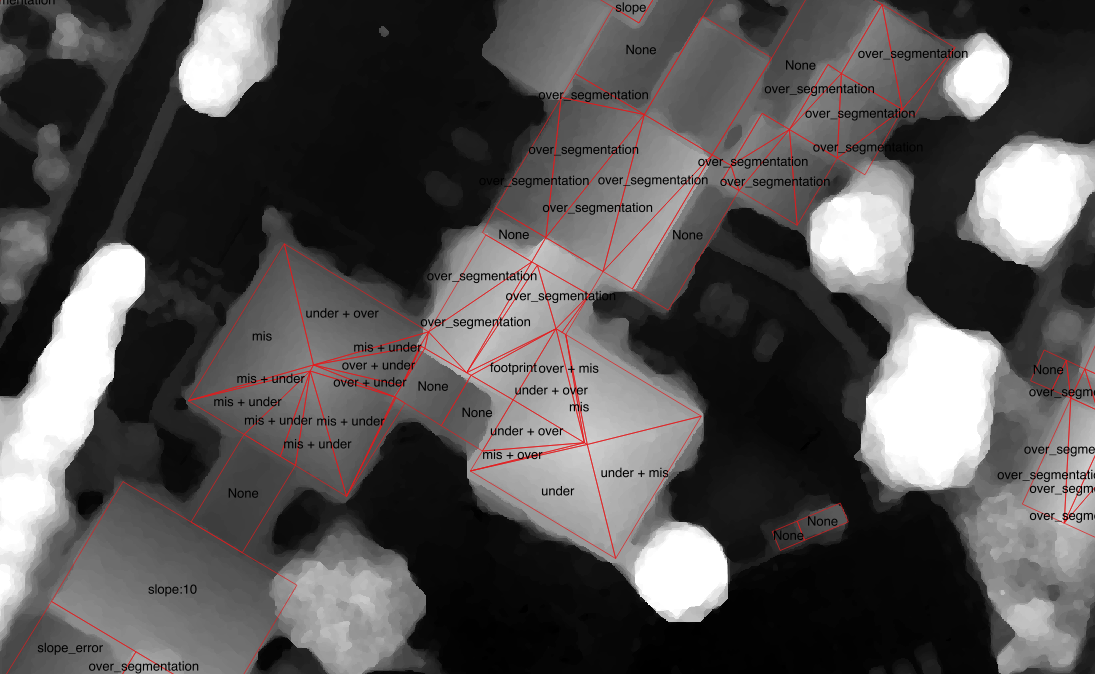
\includegraphics[width=.33\textwidth]{../images/raster/errors_sample}}
				}
				{
					\caption{Labelled errors sample.}\label{fig::errors_sample}
				}
			\end{subfloatrow}
		}
		{
			\caption{\label{fig::dataset} Labelled dataset.}
		}
	\end{figure}

	\begin{table}[H]
		\centering
		\caption{\label{my-label} }
		\begin{tabular}{|c|c|c|p{2cm}|p{2cm}|}
			\hline
			\multicolumn{1}{|l|}{Error Class}      & Ratio             & Sub Classes & Ratio among class errors & Ratio among all buildings \\ \hline
			\multirow{4}{*}{Unqualified Buildings} & \multirow{4}{*}{} &            &       &       \\ \cline{3-5}
			                                       &                   &            &       &       \\ \cline{3-5}
			                                       &                   &            &       &       \\ \cline{3-5}
			                                       &                   &            &       &       \\ \hline
			\hline
			\multirow{4}{*}{Building Error} & \multirow{4}{*}{} &            &       &       \\ \cline{3-5}
																						 &                   &            &       &       \\ \cline{3-5}
																						 &                   &            &       &       \\ \cline{3-5}
																						 &                   &            &       &       \\ \hline
      \hline
			\multirow{4}{*}{Facet Errors} & \multirow{4}{*}{} &            &       &       \\ \cline{3-5}
																						 &                   &            &       &       \\ \cline{3-5}
																						 &                   &            &       &       \\ \cline{3-5}
																						 &                   &            &       &       \\ \hline
		\end{tabular}
	\end{table}

	\begin{itemize}
		\item Ratio of \textbf{Building} errors among all errors: $0.2408$
		\begin{itemize}
			\item[-] Ratio of \textbf{Over Segmentation} errors:
			\begin{itemize}
				\item[(i).] among \textbf{Building} errors:  $0.1365$
				\item[(ii).] among all files:  $0.03287$
			\end{itemize}
			\item[-] Ratio of \textbf{Under Segmentation} errors:
			\begin{itemize}
				\item[(i).] among \textbf{Building} errors:  $0.4177$
				\item[(ii).] among all files:   $0.1006$
			\end{itemize}
			\item[-] Ratio of \textbf{Footprint} errors:
			\begin{itemize}
				\item[(i).] among \textbf{Building} errors:  $0.4839$
				\item[(ii).] among all files:  $0.1165$
			\end{itemize}
			\item[-] Ratio of \textbf{Altimetric} errors:
			\begin{itemize}
				\item[(i).] among \textbf{Building} errors:  $0.0165$
				\item[(ii).] among all files:  $0.0040$
			\end{itemize}
		\end{itemize}
		\item Ratio of \textbf{Facet} errors among all errors: $0.81657$
		\begin{itemize}
			\item[-] Ratio of \textbf{Over Segmentation} errors:
			\begin{itemize}
				\item[(i).] among \textbf{Facet} errors:  $0.8830$
				\item[(ii).] among all files:  $0.7203$
			\end{itemize}
			\item[-] Ratio of \textbf{Under Segmentation} errors:
			\begin{itemize}
				\item[(i).] among \textbf{Facet} errors:  $0.0842$
				\item[(ii).] among all files:   $0.0687$
			\end{itemize}
			\item[-] Ratio of \textbf{Mis Segmentation} errors:
			\begin{itemize}
				\item[(i).] among \textbf{Facet} errors:  $0.0806$
				\item[(ii).] among all files:  $0.0657$
			\end{itemize}
			\item[-] Ratio of \textbf{Slope} errors:
			\begin{itemize}
				\item[(i).] among \textbf{Facet} errors:  $0.0327$
				\item[(ii).] among all files:  $0.0267$
			\end{itemize}
		\end{itemize}
		\item Ratio of \textbf{Unqualified} errors among all errors: $0.0876$
		\begin{itemize}
			\item[-] Ratio of \textbf{Half Building} errors:
			\begin{itemize}
				\item[(i).] among \textbf{Unqualified} errors:  $0.8636$
				\item[(ii).] among all files:  $0.0757$
			\end{itemize}
			\item[-] Ratio of \textbf{Change Building} errors:
			\begin{itemize}
				\item[(i).] among \textbf{Unqualified} errors:  $0.0455$
				\item[(ii).] among all files:   $0.0040$
			\end{itemize}
			\item[-] Ratio of \textbf{Occlusion} errors:
			\begin{itemize}
				\item[(i).] among \textbf{Unqualified} errors:  $0.0455$
				\item[(ii).] among all files:  $0.0040$
			\end{itemize}
			\item[-] Ratio of \textbf{Unknown} errors:
			\begin{itemize}
				\item[(i).] among \textbf{Unqualified} errors:   $0.0455$
				\item[(ii).] among all files:  $0.0040$
			\end{itemize}
		\end{itemize}
	\end{itemize}


	\begin{landscape}
		\begin{figure}
			\begin{center}
				\includestandalone[mode=buildnew, scale=.78]{mind_map}
				\caption{\label{fig::mindmap_errors} Mind map summarizing the errors encountered during annotation.}
			\end{center}
		\end{figure}
	\end{landscape}

	\section{Features:}
~\\

	\subsection{Low level features:}


	The first step of computing features was to extract low level features and expose them so that I can engineer sophisticated features to train the classifiers on. In fact, For each building, I computed the facet adjacency graph --- \textit{c.f.} figure.~\ref{fig::geom_features} --- with meaningful information for each facet. I also computed the orthoprojection\footnote{Projection on the Plane $(O, \vec{\imath}, \vec{\jmath})$} of buildings and stored it in vectorial --- \textit{c.f.} figure.~\ref{fig::vector} --- and raster mode --- \textit{c.f.} figure.~\ref{fig::raster}.\\

	\thisfloatsetup{heightadjust=object}
	\begin{figure}[H]
		\ffigbox[\FBwidth]
		{
			\begin{subfloatrow}[2]
				\captionsetup{labelformat=brace, justification=raggedright}
				\ffigbox[\FBwidth]
				{\caption{Raster orthoprojection.}\label{fig::raster}}{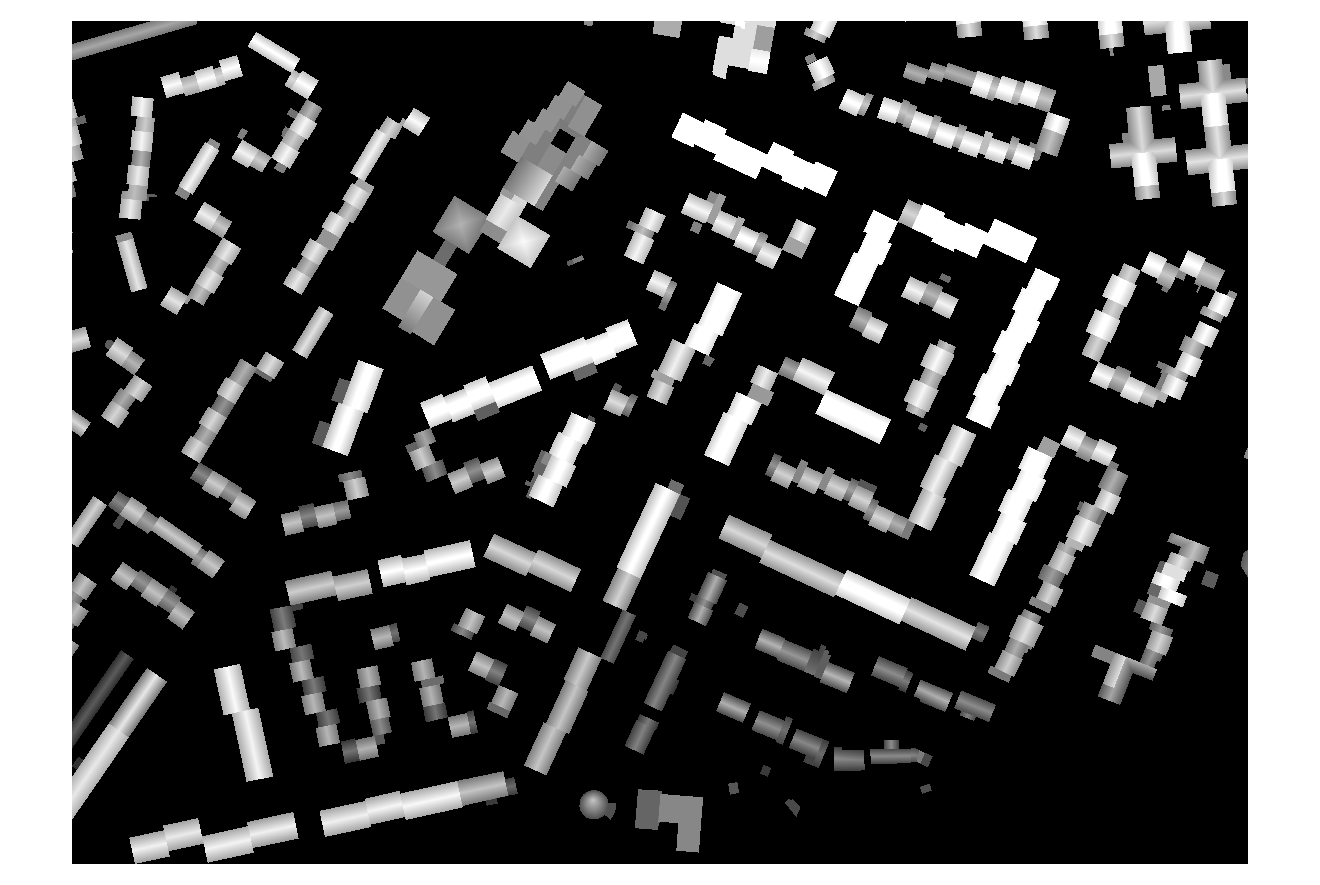
\includegraphics[width=.48\textwidth]{../images/raster/raster_projection}}
				\ffigbox[\FBwidth]{\caption{Vector orthoprojections (in transparent blue).}\label{fig::vector}}{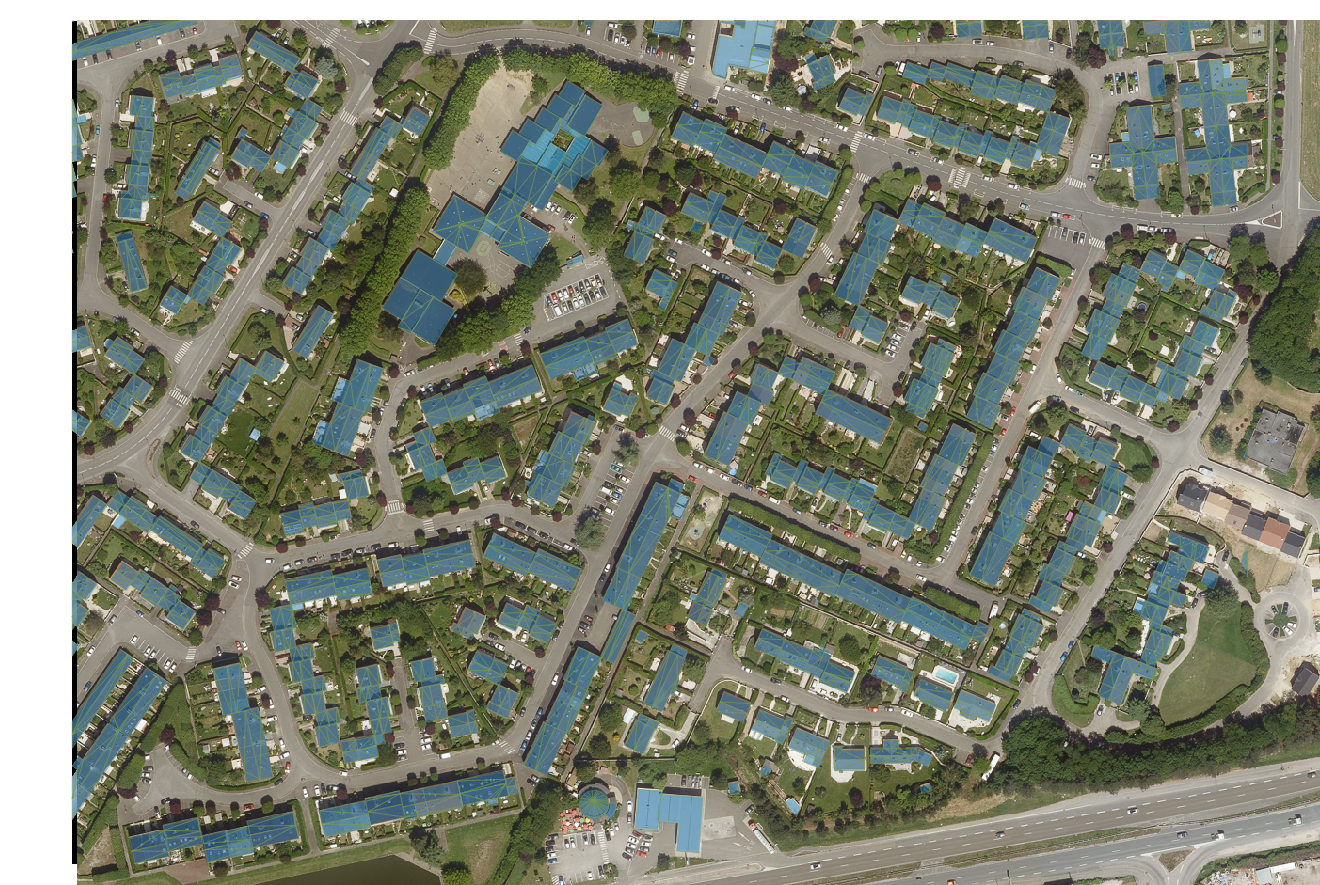
\includegraphics[width=.48\textwidth]{../images/raster/vector_projection}}
			\end{subfloatrow}
		}
		{
			\caption{\label{fig::orthoproj}Scene orthoprojections.}
		}
	\end{figure}

	\begin{figure}[H]
		\includestandalone[mode=buildnew, scale=.78]{dual_features}
		\caption{\label{fig::geom_features} Low level geometric features per building.}
	\end{figure}
	\clearpage

	\subsection{Mid level features:}
~\\

	The previous features are raw and not useful for classification. As a first
	step, in order to establish a baseline for the qualification, I choose simple
	features that can be classed as follows:
	\begin{itemize}
		\item[(i).] Geometric --- or intrinsic --- features: based on the graph adjacency features and the vector orthoprojections, I tried the feature vector per building in equation.~\ref{eq::feature_vec}:
		\begin{equation}\label{eq::feature_vec}
			\text{feature\_vector} = \begin{bmatrix}
				statistics(degree_{facets})\\
				statistics(areas_{facets})\\
				statistics(centroid_{facets})\\
				statistics(normal_{facets})\\
				statistics(nomal\_with\_relations_{facets})
		\end{bmatrix}
		\end{equation}
		where:
		\begin{equation}
			statistics: property \mapsto \begin{bmatrix}
			\max_{facets}(property)\\
			\min_{facets}(property)\\
			mean_{facets}(property)\\
			median_{facets}(property)
		\end{bmatrix}
		\end{equation}
		\item[(ii).] Altimetric features: using the raster projections and the provided DSM, I computed the difference and used the its histogram as a feature vector. I can also try Bredif's method for DSM roof fitting later on.
		\item[(iii.)] Image features: left for later.
	\end{itemize}

	For now, I have focused on geometric features and altimetic features to complete the whole classification pipeline.The graph kernel methods and ortho image features are left for later. I should also grow my labelled datasets and invistigate other regions by active learning: transforming the pipeline to an active setting.

	\section{Experiments:}
~\\
	\subsection{Features visualization:}

	I tried visualizing features by reducing their dimensions using PCA. In figure , we can see how

	I am trying also to cluster the features in between $9$ --- number of all subclasses --- and $3$ --- number of Coarse classes --- clusters. The idea is to see if features can be interpreted and are well defined or we are overfitting during classification.

	\subsection{Classification results:}

	The classification pipeline is subdivided into two phases:

	\begin{itemize}
		\item[(i).] Binary classification: the idea is to use geometric features to predict the unqualified builings which are to be discarded. They cannot be classified an can be determined also by the operator;
		\item[(ii).] Coarse Multi classification: classifies qualified buildings by the error classes: 'None', 'Building error', 'Facet error'. We can observe the results of cross validated \textit{Random Forests} and \textit{SVM} in . We can also observe how facet relations play a big role in the classification.
	\end{itemize}

	The work is still at its begining. I need to classify now on subclasses and try to link the results back to real building in QGIS.

	\section*{Attachments:}
	\begin{itemize}
		\item[-] You can checkout the preprocessing code on
		\href{https://github.com/ethiy/proj.city}{Github}.
		\item[-] You can also check the feature extraction and classification code
		\href{https://github.com/ethiy/qualcity}{here}.
	\end{itemize}

\end{document}
